%%%%%%%%%%%%%%%%%%%%%%%%%%%%%%%%%%%%%%%%%%%
%
% From a template maintained at https://github.com/jamesrobertlloyd/cbl-tikz-poster
%
% Code near the top should be fairly standard and not need to be changed
%  - except for the document class
% Code lower down is more likely to be customised
%
%%%%%%%%%%%%%%%%%%%%%%%%%%%%%%%%%%%%%%%%%%%
\documentclass[landscape,a0b,final,a4resizeable]{include/a0poster}

\usepackage{multicol}
\usepackage{color}
\usepackage{morefloats}
\usepackage[pdftex]{graphicx}
\usepackage{rotating}
\usepackage{amsmath, amsthm, amssymb, bm}
\usepackage{array}
\usepackage{booktabs}
\usepackage{multirow}
\usepackage{hyperref}
\usepackage{include/picins}
\usepackage{tikz}
\usetikzlibrary{shapes.geometric,arrows,chains,matrix,positioning,scopes,calc}
\tikzstyle{mybox} = [draw=white, rectangle]
\definecolor{darkblue}{rgb}{0,0.08,0.45}
\definecolor{blue}{rgb}{0,0,1}
\usepackage{dsfont}
\usepackage{wrapfig}
\ProvidesPackage{preamble}

\usepackage{url}
\usepackage{array}
\usepackage{amsmath,amssymb,amsfonts,textcomp,amsthm}
\usepackage{booktabs}
\usepackage{relsize}
\usepackage{nicefrac}
\usepackage{graphicx}
\usepackage{rotating}
\usepackage{nth}
\usepackage{acronym}
\usepackage{bm}
%\usepackage{caption} \DeclareCaptionType{copyrightbox}
\usepackage{footnote}
\usepackage{color}

\usepackage{tabularx}
\newcolumntype{x}[1]{>{\centering\arraybackslash\hspace{0pt}}m{#1}}
\newcommand{\tabbox}[1]{#1}

\usepackage{hyperref}
\definecolor{mydarkblue}{rgb}{0,0.08,0.45}
\hypersetup{
    pdftitle={},
    pdfauthor={},
    pdfsubject={},
    pdfkeywords={},
    pdfborder=0 0 0,
    pdfpagemode=UseNone,
    colorlinks=true,
    linkcolor=mydarkblue,
    citecolor=mydarkblue,
    filecolor=mydarkblue,
    urlcolor=mydarkblue,
    pdfview=FitH}

\newcommand{\asdf}{$^{\textnormal{th}}$}

\newcommand{\binarysum}{\sum_{\bf{x} \in \{0,1\}^D}}
\newcommand{\expect}{\mathbb{E}}
\newcommand{\expectargs}[2]{\mathbb{E}_{#1} \left[ {#2} \right]}
\newcommand{\var}{\mathbb{V}}
\newcommand{\varianceargs}[2]{\mathbb{V}_{#1} \left[ {#2} \right]}
\newcommand{\variance}{\mathbb{V}}
\newcommand{\cov}{\operatorname{cov}}
\newcommand{\Cov}{\operatorname{Cov}}
\newcommand{\covarianceargs}[2]{\Cov_{#1} \left[ {#2} \right]}
\newcommand{\colvec}[2]{\left[ \begin{array}{c} {#1} \\ {#2} \end{array} \right]}
\newcommand{\tbtmat}[4]{\left[ \begin{array}{cc} {#1} & {#2} \\ {#3} & {#4} \end{array} \right]}

%\newcommand{\covskinny}[2]{\var\!\left(#1\middle\vert#2\right)} 

\newcommand{\acro}[1]{\textsc{#1}}
%\newcommand{\vect}[1]{\boldsymbol{#1}}
%\newcommand{\vect}[1]{{\bf{#1}}}
\newcommand{\mat}[1]{\mathbf{#1}}
\newcommand{\pderiv}[2]{\frac{\partial #1}{\partial #2}}
\newcommand{\npderiv}[2]{\nicefrac{\partial #1}{\partial #2}}

\newcommand{\pha}{^{\phantom{:}}}

\newcommand{\argmin}{\operatornamewithlimits{argmin}}
\newcommand{\argmax}{\operatornamewithlimits{argmax}}

% The following designed for probabilities with long arguments

\newcommand{\Prob}[2]{P\!\left(\,#1\;\middle\vert\;#2\,\right)}
\newcommand{\ProbF}[3]{P\!\left(\,#1\!=\!#2\;\middle\vert\;#3\,\right)}
\newcommand{\p}[2]{p\!\left(#1\middle\vert#2\right)}
\newcommand{\po}[1]{p\!\left(#1\right)}
\newcommand{\pF}[3]{p\!\left(\,#1\!=\!#2\;\middle\vert\;#3\,\right)} 
\newcommand{\mean}[2]{{m}\!\left(#1\middle\vert#2\right)}
%\newcommand{\novmean}[2]{{m}\!\left(#1\middle\vert#2\right)}
%\newcommand{\novcov}[2]{\var\!\left(#1\middle\vert#2\right)}
%\newcommand{\cov}[2]{\var\!\left(#1\middle\vert#2\right)} 
%\newcommand{\pskinny}[2]{p\!\left(#1\;\middle\vert\;#2\right)}
%\newcommand{\meanskinny}[2]{{m}\!\left(#1\middle\vert#2\right)}
%\newcommand{\covskinny}[2]{\var\!\left(#1\middle\vert#2\right)} 

\newcommand{\vI}{\mat{I}}
\newcommand{\vX}{\mat{X}}
\newcommand{\vY}{\mat{Y}}
\newcommand{\vZ}{\mat{Z}}
\newcommand{\vK}{\mat{K}}
\newcommand{\vs}{\vect{s}}
\newcommand{\va}{\vect{a}}
\newcommand{\vA}{\vect{A}}
\newcommand{\vb}{\vect{b}}
\newcommand{\vB}{\mat{B}}
\newcommand{\vR}{\mat{R}}
\newcommand{\vS}{\mat{S}}
\newcommand{\vu}{\vect{u}}
\newcommand{\vk}{\vect{k}}
\newcommand{\vc}{\vect{c}}
\newcommand{\vC}{\mat{C}}
\newcommand{\vw}{\vect{w}}
\newcommand{\vx}{\vect{x}}
\newcommand{\vy}{\vect{y}}
\newcommand{\vz}{\vect{z}}
\newcommand{\vmu}{\vect{\mu}}
\newcommand{\vpi}{\vect{\pi}}
\newcommand{\vphi}{\vect{\phi}}
\newcommand{\vSigma}{\mat{\Sigma}}
\newcommand{\vtheta}{\vect{\theta}}
\newcommand{\vl}{\vect{l}}
\newcommand{\vq}{\vect{q}}
\newcommand{\vf}{\vect{f}}
\newcommand{\vg}{\vect{g}}
\newcommand{\vell}{\vect{\ell}}
\newcommand{\ve}{\vect{\epsilon}}
\newcommand{\vzero}{\vect{0}}
\newcommand{\vone}{\vect{1}}

\newcommand{\He}{\mathcal{H}}
\newcommand{\normx}[2]{\left\|#1\right\|_{#2}}
\newcommand{\Hnorm}[1]{\normx{#1}{\He}}
\newcommand{\mmd}{{\rm MMD}}


\newcommand{\mf}{\bar{\vf}}

\newcommand{\st}{_\star}

\newcommand{\inv}{^{{\mathsmaller{-1}}}}
\newcommand{\tohalf}{^{{\mathsmaller{\nicefrac{1}{2}}}}}

\newcommand{\Normal}{\mathcal{N}}
\newcommand{\N}[3]{\mathcal{N}\!\left(#1|#2,#3\right)}
\newcommand{\Nt}[2]{\mathcal{N}\!\left(#1,#2\right)}
\newcommand{\bN}[3]{\mathcal{N}\big(#1|#2,#3\big)}
\newcommand{\boldN}[3]{\text{\textbf{\mathcal{N}}}\big(#1;#2,#3\big)}
\newcommand{\ones}[1]{\mat{1}_{#1}}
\newcommand{\eye}[1]{\mat{E}_{#1}}
\newcommand{\tra}{{^\ensuremath{\mathsf{T}}}}
\newcommand{\trace}{\operatorname{tr}}
\newcommand{\deq}{:=}
\newcommand{\degree}{^\circ}

\newcommand{\GPt}[2]{\mathcal{GP}\!\left(#1,#2\right)}

\DeclareMathOperator{\chol}{chol}
\DeclareMathOperator{\diag}{diag}

\newcommand{\gp}{{\acro{gp}}}
\newcommand{\gplvm}{{\acro{gp-lvm}}}
\newcommand{\bmc}{{\acro{bmc}}}
\newcommand{\bq}{{\acro{bq}}}
\newcommand{\sbq}{{\acro{sbq}}}

\newenvironment{narrow}[2]{%
  \begin{list}{}{%
  \setlength{\topsep}{0pt}%
  \setlength{\leftmargin}{#1}%
  \setlength{\rightmargin}{#2}%
  \setlength{\listparindent}{\parindent}%
  \setlength{\itemindent}{\parindent}%
  \setlength{\parsep}{\parskip}}%
\item[]}{\end{list}}



\newcommand{\dist}{\ \sim\ }
\def\given{\,|\,}

% Table stuff
\newcolumntype{C}[1]{>{\centering\let\newline\\\arraybackslash\hspace{0pt}}m{#1}}
\newcolumntype{L}[1]{>{\raggedright\let\newline\\\arraybackslash\hspace{0pt}}m{#1}}
\newcolumntype{R}[1]{>{\raggedleft\let\newline\\\arraybackslash\hspace{0pt}}m{#1}}


\def\ie{i.e.\ }
\def\eg{e.g.\ }
\def\iid{i.i.d.\ }
%\def\simiid{\sim_{\mbox{\tiny iid}}}
\def\simiid{\overset{\mbox{\tiny iid}}{\sim}}
\def\eqdist{\stackrel{\mbox{\tiny d}}{=}}
\newcommand{\distas}[1]{\mathbin{\overset{#1}{\kern\z@\sim}}}

\def\Reals{\mathbb{R}}

\def\Uniform{\mbox{\rm Uniform}}
\def\Bernoulli{\mbox{\rm Bernoulli}}
\def\GP{\mathcal{GP}}
\def\GPLVM{\mathcal{GP-LVM}}

% Kernel stuff

\def\inputVar{x}
\def\InputVar{X}
\def\InputSpace{\mathcal{X}}
\def\outputVar{y}
\def\OutputSpace{\mathcal{Y}}
\def\function{f}
\def\kernel{k}
\def\KernelMatrix{K}
\def\SumKernel{\sum}
\def\ProductKernel{\prod}
\def\expression{e}

\def\SE{\acro{SE}}
\def\Per{\acro{Per}}
\def\RQ{\acro{RQ}}
\def\Lin{\acro{Lin}}

\def\subexpr{{\cal S}}
\def\baseker{{\cal B}}
\def\numWinners{k}

\newcommand{\kSE}{{\acro{SE}}}
\newcommand{\kPer}{{\acro{Per}}}
\newcommand{\kLin}{{\acro{Lin}}}
\newcommand{\kRQ}{{\acro{RQ}}}


% Proof stuff
\theoremstyle{plain}
\newtheorem{theorem}{Theorem}[section]
\newtheorem{lemma}[theorem]{Lemma}
\newtheorem{prop}[theorem]{Proposition}
\newtheorem*{cor}{Corollary}

%%%%%%%%%%%%%%%%%%%%%%%%%%%%%%%%%%%%%%%%%%%
%
% myfig
%
% \myfig - replacement for \figure
% necessary, since in multicol-environment 
% \figure won't work        
%                 
%%%%%%%%%%%%%%%%%%%%%%%%%%%%%%%%%%%%%%%%%%%

\newcommand{\myfig}[3][0]{
\begin{center}
  \vspace{1.5cm}
  \includegraphics[width=#3\hsize,angle=#1]{#2}
  \nobreak\medskip
\end{center}}

%%%%%%%%%%%%%%%%%%%%%%%%%%%%%%%%%%%%%%%%%%%
%
% mycaption                
%
% \mycaption - replacement for \caption
% necessary, since in multicol-environment \figure and
% therefore \caption won't work
%
%%%%%%%%%%%%%%%%%%%%%%%%%%%%%%%%%%%%%%%%%%%

%\newcounter{figure}
\setcounter{figure}{1}
\newcommand{\mycaption}[1]{
  \vspace{0.5cm}
  \begin{quote}
    {{\sc Figure} \arabic{figure}: #1}
  \end{quote}
  \vspace{1cm}
  \stepcounter{figure}
}

%%%%%%%%%%%%%%%%%%%%%%%%%%%%%%%%%%%%%%%%%%%
%
% Some standard colours
%
%%%%%%%%%%%%%%%%%%%%%%%%%%%%%%%%%%%%%%%%%%%

\definecolor{camlightblue}{rgb}{0.601 , 0.8, 1}
\definecolor{camdarkblue}{rgb}{0, 0.203, 0.402}
\definecolor{camred}{rgb}{1, 0.203, 0}
\definecolor{camyellow}{rgb}{1, 0.8, 0}
\definecolor{lightblue}{rgb}{0, 0, 0.80}
\definecolor{white}{rgb}{1, 1, 1}
\definecolor{whiteblue}{rgb}{0.80, 0.80, 1}

%%%%%%%%%%%%%%%%%%%%%%%%%%%%%%%%%%%%%%%%%%%
%
% Some look and feel definitions
%
%%%%%%%%%%%%%%%%%%%%%%%%%%%%%%%%%%%%%%%%%%%

\setlength{\columnsep}{0.03\textwidth}
\setlength{\columnseprule}{0.0018\textwidth}
\setlength{\parindent}{0.0cm}

%%%%%%%%%%%%%%%%%%%%%%%%%%%%%%%%%%%%%%%%%%%
%
% \mysection - replacement for \section*
% 
% Puts a pretty box around some text
% TODO - any other thoughts for what this box should look like
%
%%%%%%%%%%%%%%%%%%%%%%%%%%%%%%%%%%%%%%%%%%%

\tikzstyle{mysection} = [rectangle, 
			draw=none, 
			shade, 
			outer color=camlightblue!30,
			inner color=camlightblue!30,
			text width=0.965\columnwidth,
			text centered,
			rounded corners=20pt,
			minimum height=0.09\columnwidth]

\newcommand{\mysection}[1]
{
\begin{center}
  \begin{tikzpicture}
    \node[mysection] {\sffamily\bfseries\LARGE#1};
  \end{tikzpicture}
\end{center}
}

%%%%%%%%%%%%%%%%%%%%%%%%%%%%%%%%%%%%%%%%%%%
%
% Set the font
%
% TODO - Not sure what a canonical choice is - feel free to modify
%
%%%%%%%%%%%%%%%%%%%%%%%%%%%%%%%%%%%%%%%%%%%

\renewcommand{\familydefault}{cmss}
\sffamily

%%%%%%%%%%%%%%%%%%%%%%%%%%%%%%%%%%%%%%%%%%%%%%%%%%%%
%%%               Background                     %%%
%%%%%%%%%%%%%%%%%%%%%%%%%%%%%%%%%%%%%%%%%%%%%%%%%%%%

\newcommand{\background}[3]{
  %\definecolor{cgradbegin}{#1}
  %\definecolor{cgradend}{#2}
 % \psframe[fillstyle=gradient,gradend=cgradend,
 % gradbegin=cgradbegin,gradmidpoint=#3](0.,0.)(1.\textwidth,-1.\textheight)
}




%%%%%%%%%%%%%%%%%%%%%%%%%%%%%%%%%%%%%%%%%%%%%%%%%%%%
%%%                pcolumn                       %%%
%%%%%%%%%%%%%%%%%%%%%%%%%%%%%%%%%%%%%%%%%%%%%%%%%%%%

\newenvironment{pcolumn}[1]{
  \begin{minipage}{#1\textwidth}
  \begin{center}
}{
  \end{center}
  \end{minipage}
}



%%%%%%%%%%%%%%%%%%%%%%%%%%%%%%%%%%%%%%%%%%%%%%%%%%%%
%%%                pbox                          %%%
%%%%%%%%%%%%%%%%%%%%%%%%%%%%%%%%%%%%%%%%%%%%%%%%%%%%

\definecolor{lcolor}{rgb}{0, 0, 0.80}
\definecolor{gcolor1}{rgb}{1, 1, 1}
\definecolor{gcolor2}{rgb}{.80, .80, 1}

  % \def\fc{fillcolor}
  % \def\getfc #1=#2\par{\def\ffc{#1} \ifx\ffc\fc #2\fi} 
  % \def\getfillcolor #1,#2\par{\getfc #1\par \getfc #2\par}

 %  \newcommand{\psshadowbox}[2]{%[2][magenta]{
%      \fbox{Input arg: #1}
%      \fbox{#1} 
%      \fbox {\getfillcolor #1\par}
%      \def\col{\getfillcolor #1\par}
 
%      \let\coll=\col
%       \coll
 %     \colorbox{\col}{#2}
%       \mbox
   %   \coloredshadowbox{black}{\coll}{#2}
%   }

\newcommand{\pbox}[4]{
%\psshadowbox[#3]{
%\fbox{
\mbox{
\begin{minipage}[t][#2][t]{#1}
#4
\end{minipage}
}%}
}

%%%%%%%%%%%%%%%%%%%%%%%%%%%%%%%%%%%%%%%%%%%
%
% Poster environment
%
% Centres everything and can be used to define the width of the content
%
%%%%%%%%%%%%%%%%%%%%%%%%%%%%%%%%%%%%%%%%%%%

\newenvironment{poster}{
  \begin{center}
  \begin{minipage}[c]{\textwidth}
}{
  \end{minipage}
  \end{center}
}

\def\newarrow{\mbox{\begin{tikzpicture}
             \useasboundingbox{(-3pt,-4.5pt) rectangle (19pt,1pt)};
             \draw[->] (0,-0.07)--(17pt,-0.07);\end{tikzpicture}}}


\usepackage{algorithm}% http://ctan.org/pkg/algorithms
\usepackage[noend]{algpseudocode} % http://ctan.org/pkg/algorithmicx

% Custom notation
% HUMBLE WORDS: shown slightly smaller when in normal text
\makeatletter
\newlength{\nonHumbleHeight}
\def\@humbleformat#1{{\settoheight{\nonHumbleHeight}{#1}\resizebox{!}{0.94\nonHumbleHeight}{#1}}}
\def\humble#1{\@humbleformat{#1}}
\makeatother
\newcommand{\logowidth}{0.099\textwidth}  % width mauna decomp
\newtheorem*{theorem*}{Theorem}


\begin{document}
\begin{poster}
% Potentially add some space at the top of the poster
\vspace{0\baselineskip}

%%% Header
\begin{center}
\begin{pcolumn}{0.99}

\pbox{0.99\textwidth}{}{linewidth=2mm,framearc=0.3,linecolor=camdarkblue,fillstyle=gradient,gradangle=0,gradbegin=white,gradend=white,gradmidpoint=1.0,framesep=1em}{
%%% U of T Logo
\begin{minipage}[c]{9cm}
  \begin{center}
    
\includegraphics[width=9cm]{badges/toronto.png}
    %
\includegraphics[width=10cm]{badges/uot_text.pdf}
  \end{center}
\end{minipage}
%%% Title
\begin{minipage}[c][9cm][c]{0.76\textwidth}
  \begin{center}
    {\sffamily \VeryHuge \textbf{Stochastic Hyperparameter Optimization with Hypernets}}\\[10mm]
    {\huge\sffamily \Huge Jonathan Lorraine, David Duvenaud\\[7.5mm]
    \huge\sffamily \Huge University of Toronto\\[7.5mm]%\texttt{\{ti242, dkd23, zoubin\}@cam.ac.uk}
    }
  \end{center}
\end{minipage}
%
% Other Logo logo
%\begin{minipage}[c]{\logowidth}
%  \begin{flushright}
%    \includegraphics[width=8cm,trim=2em 0em 2em 2em, clip]{badges/harvard}
%  \end{flushright}
%\end{minipage}
%
}
\end{pcolumn}
\end{center}

\vspace*{2.5cm}
\large

%%%%%%%%%%%%%%%%%%%%%%%%%%%%%%%%%%%%%%%%%%%%%%%%%%%%%%%%%%%%%%%%%%%%%%
%%% Beginning of Document
%%%%%%%%%%%%%%%%%%%%%%%%%%%%%%%%%%%%%%%%%%%%%%%%%%%%%%%%%%%%%%%%%%%%%%

\begin{multicols}{3}

\mysection{Main Idea}

%TODO: CLIP LEGEND ON FIRST PICTURE
%TODO: ADD THE TWO MANIFOLD PICTURES
%TODO: FIX SPACING
%TODO: MAKE SLIDE
%TODO: MAIL TO DAVID FOR COMMNTS

\begin{itemize}
	\item Machine learning models often nest optimization of model weights in the optimization of hyperparameters.
	\item We collapse the nested optimization into joint optimization by training a neural network to output optimal weights for each hyperparameter.
	\item The method converges to locally optimal weights and hyperparameters for large hypernets and effectively tunes thousands of hyperparameters.
\end{itemize}

\begin{minipage}[c]{36cm}
\begin{center}
	%\vspace{-1.3cm}
	%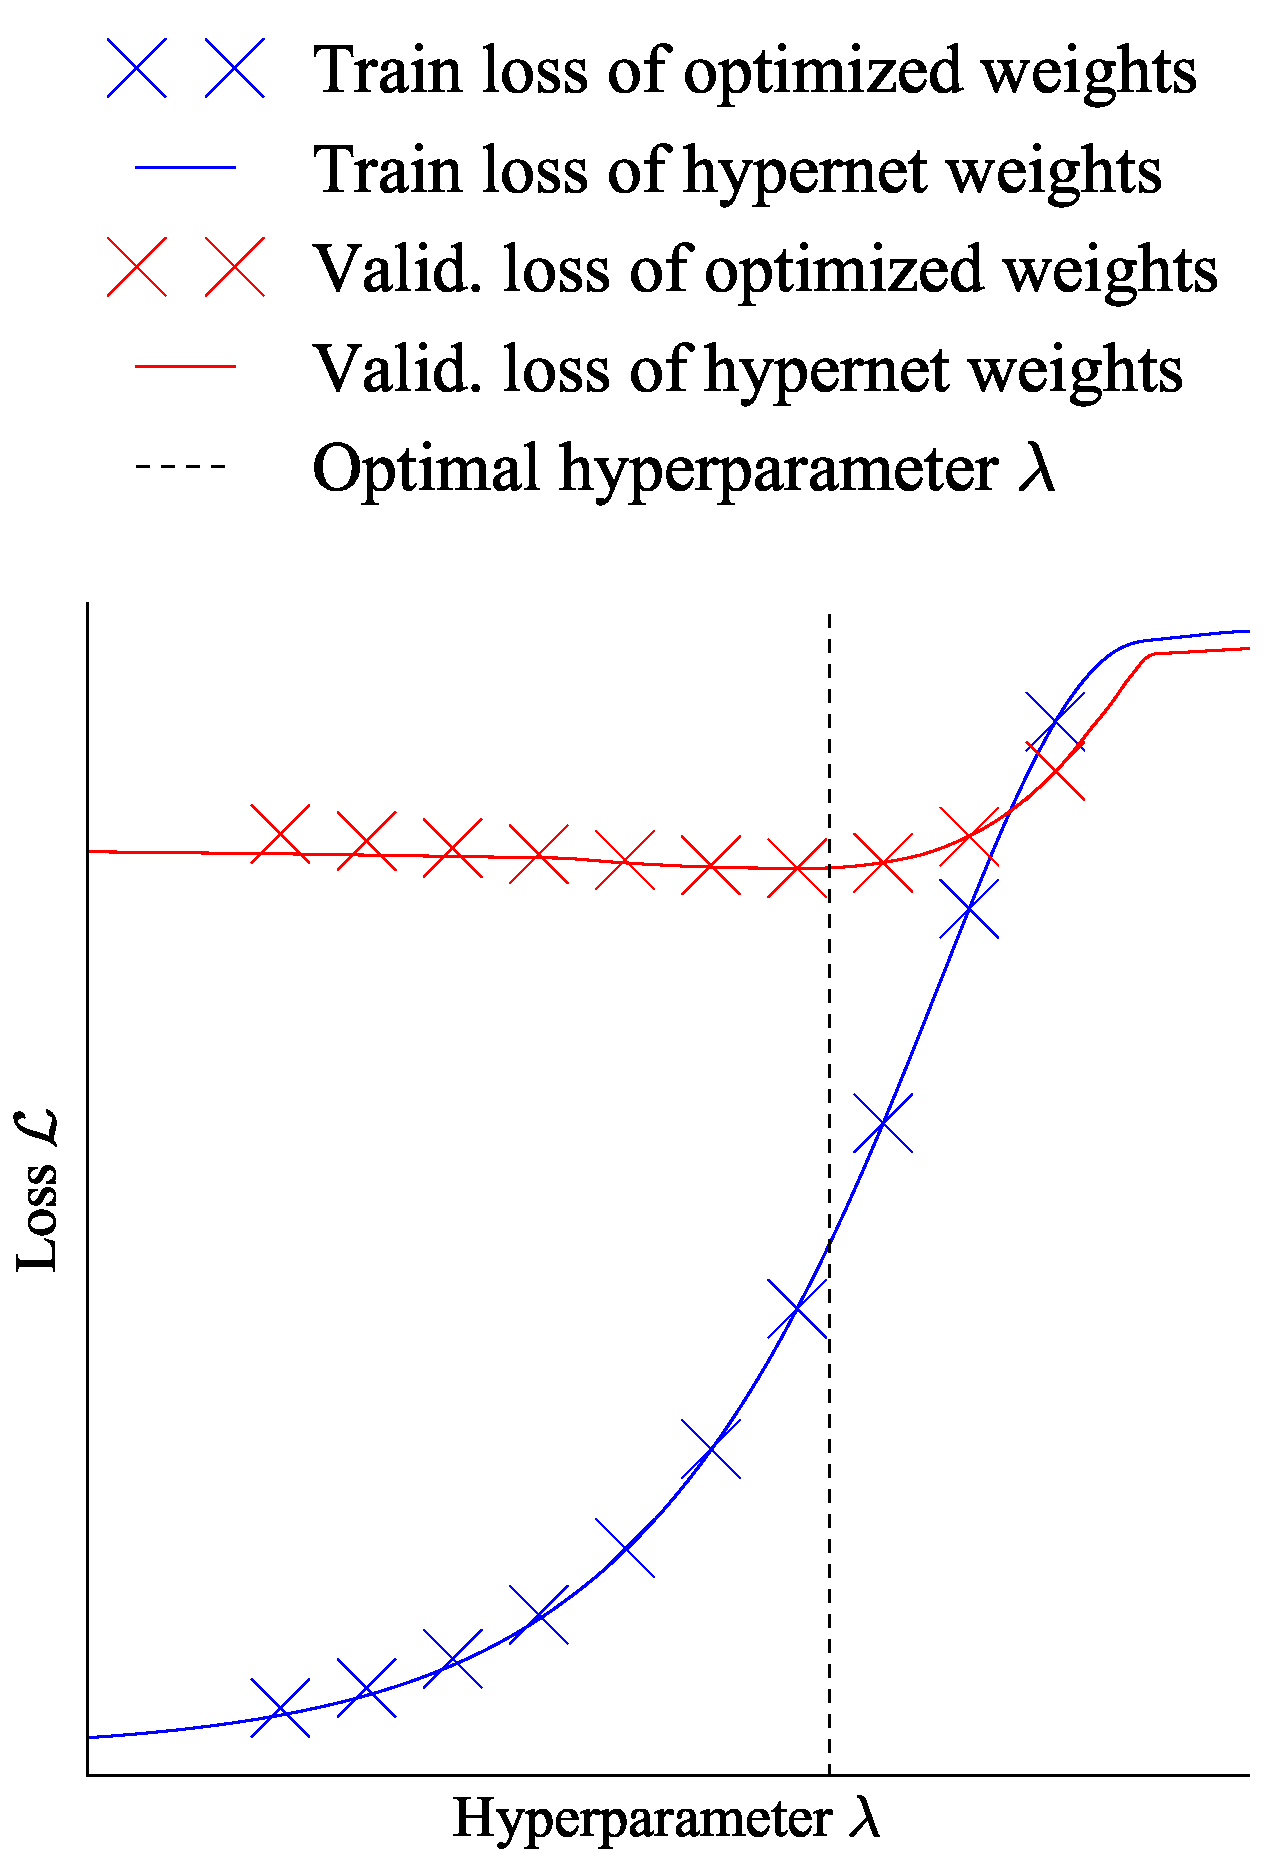
\includegraphics[trim={0 22cm 0 0},clip,height=6cm]{figures/hypernets_global_small.pdf}
	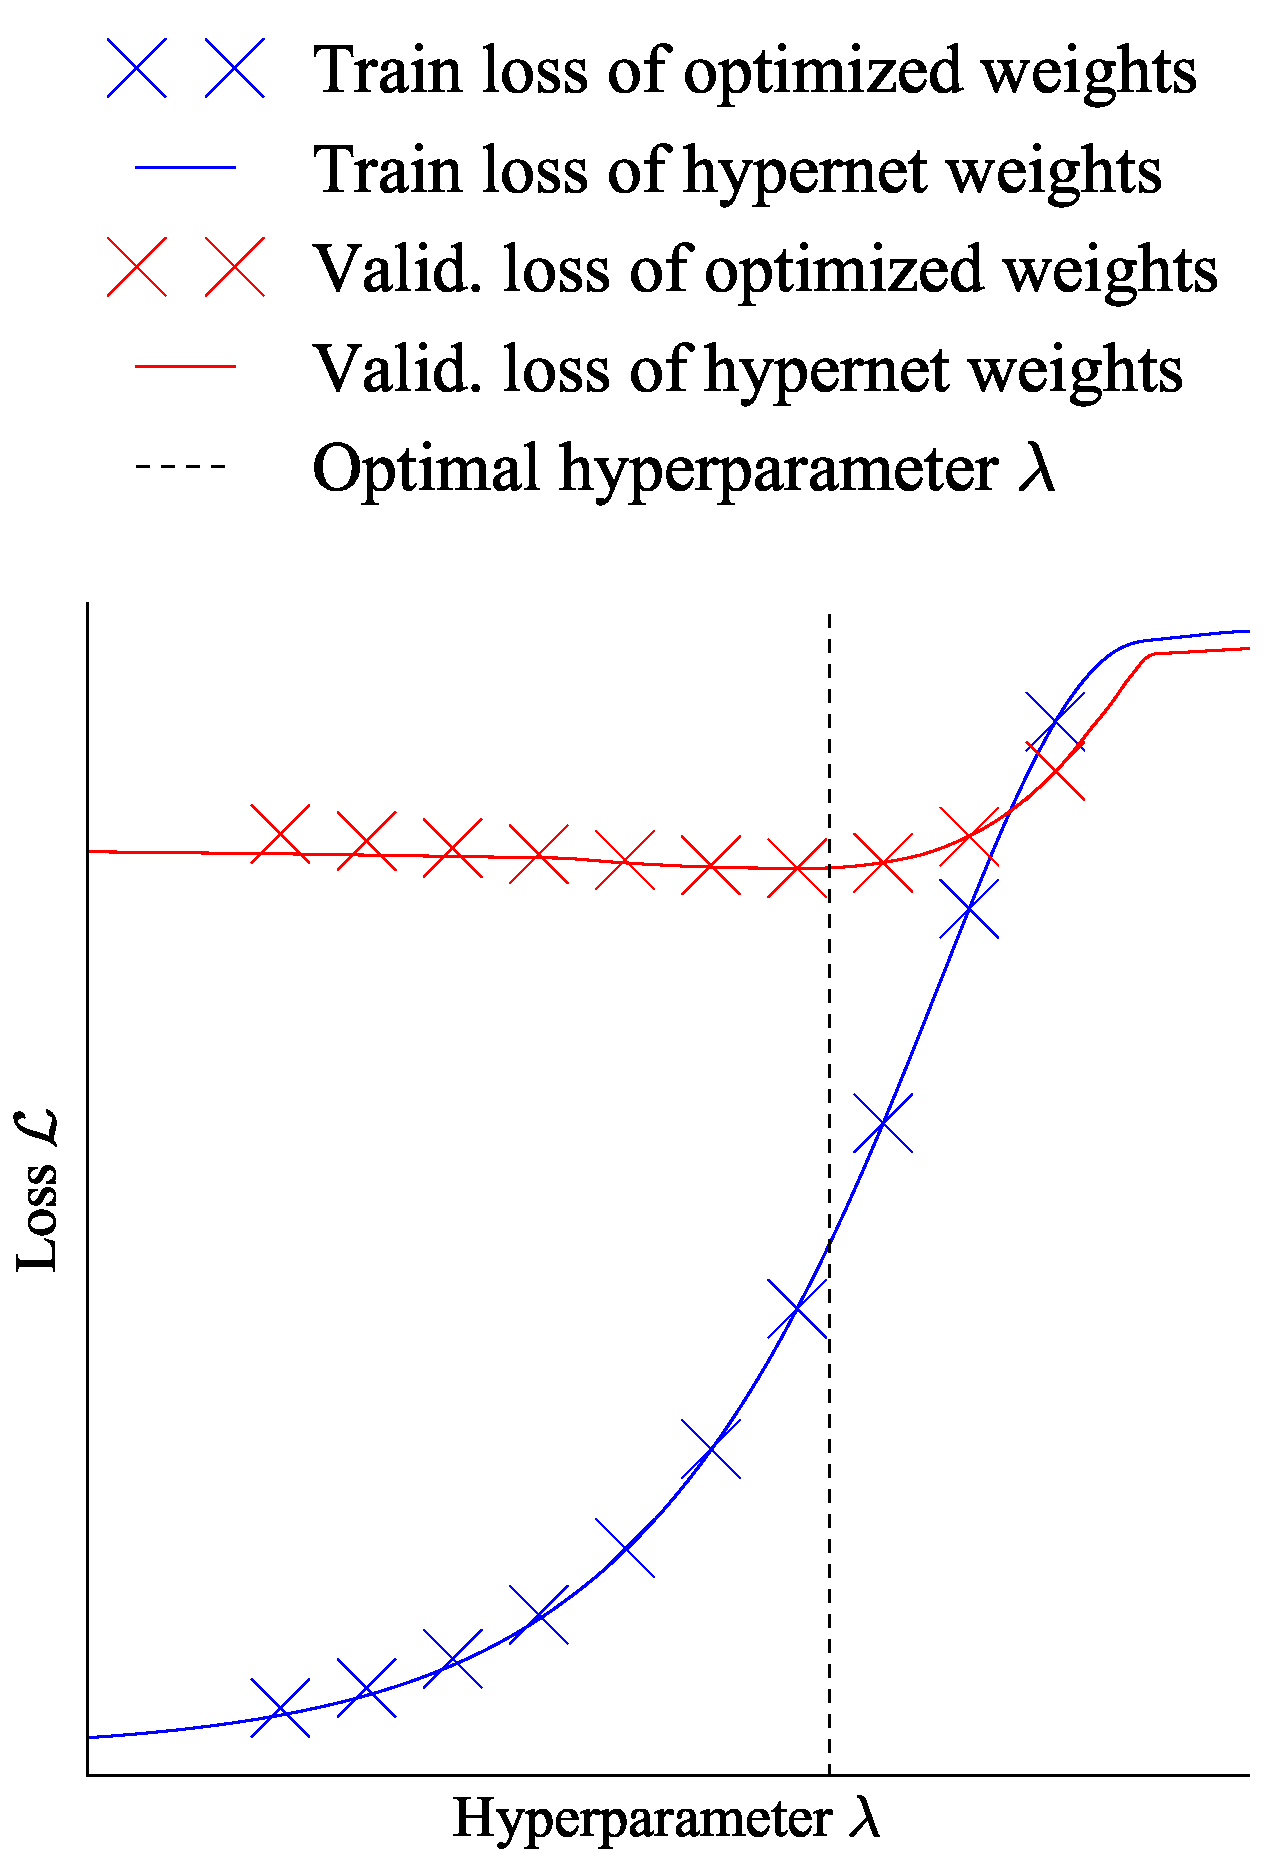
\includegraphics[trim={0 0 0 9cm},clip,width=10.5cm]{figures/hypernets_global_small.pdf}
	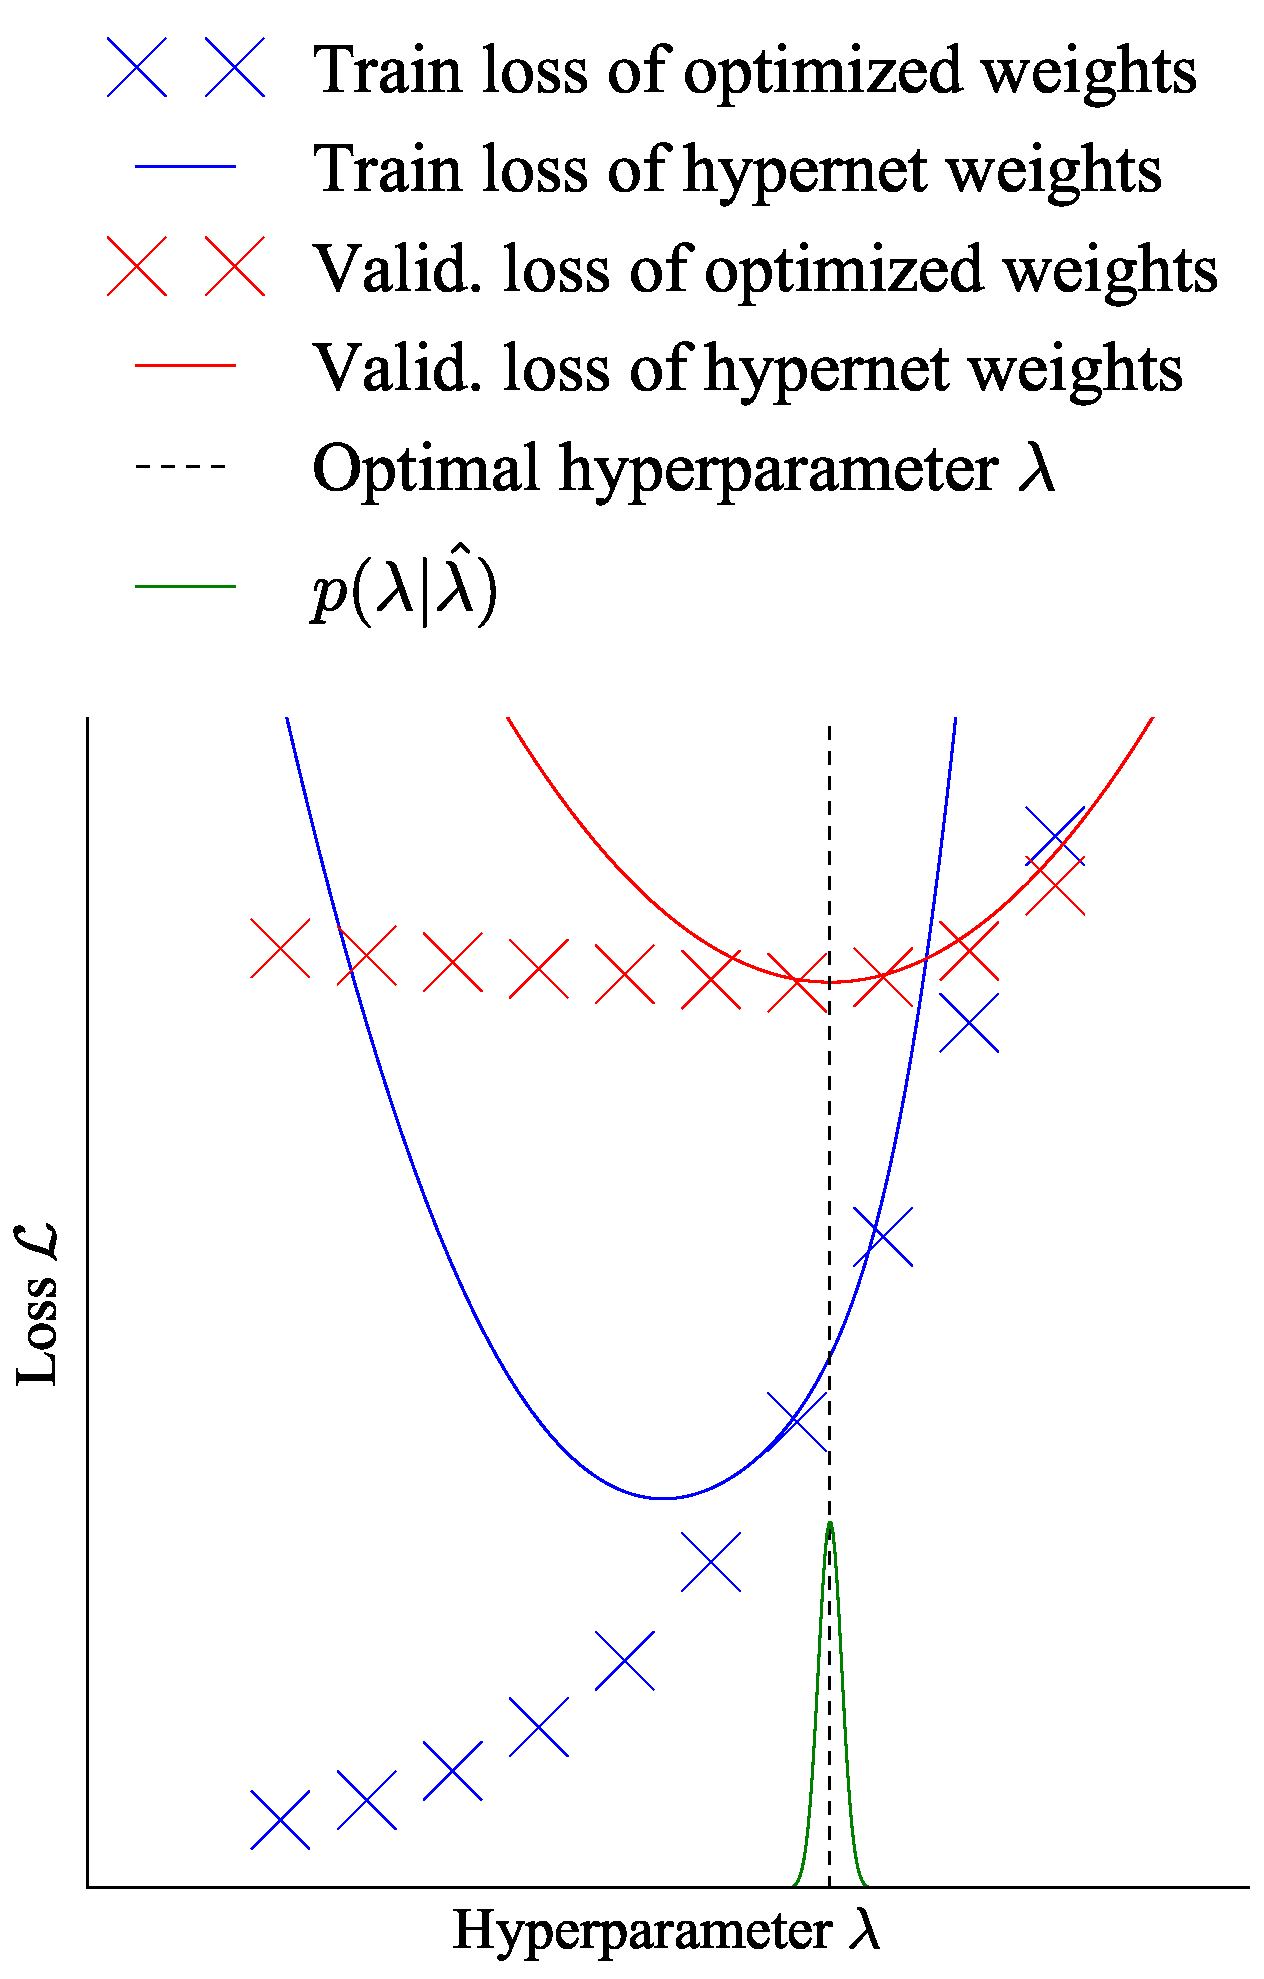
\includegraphics[trim={0 0 0 11cm},clip,width=10.5cm]{figures/hypernets_local_small.pdf}
	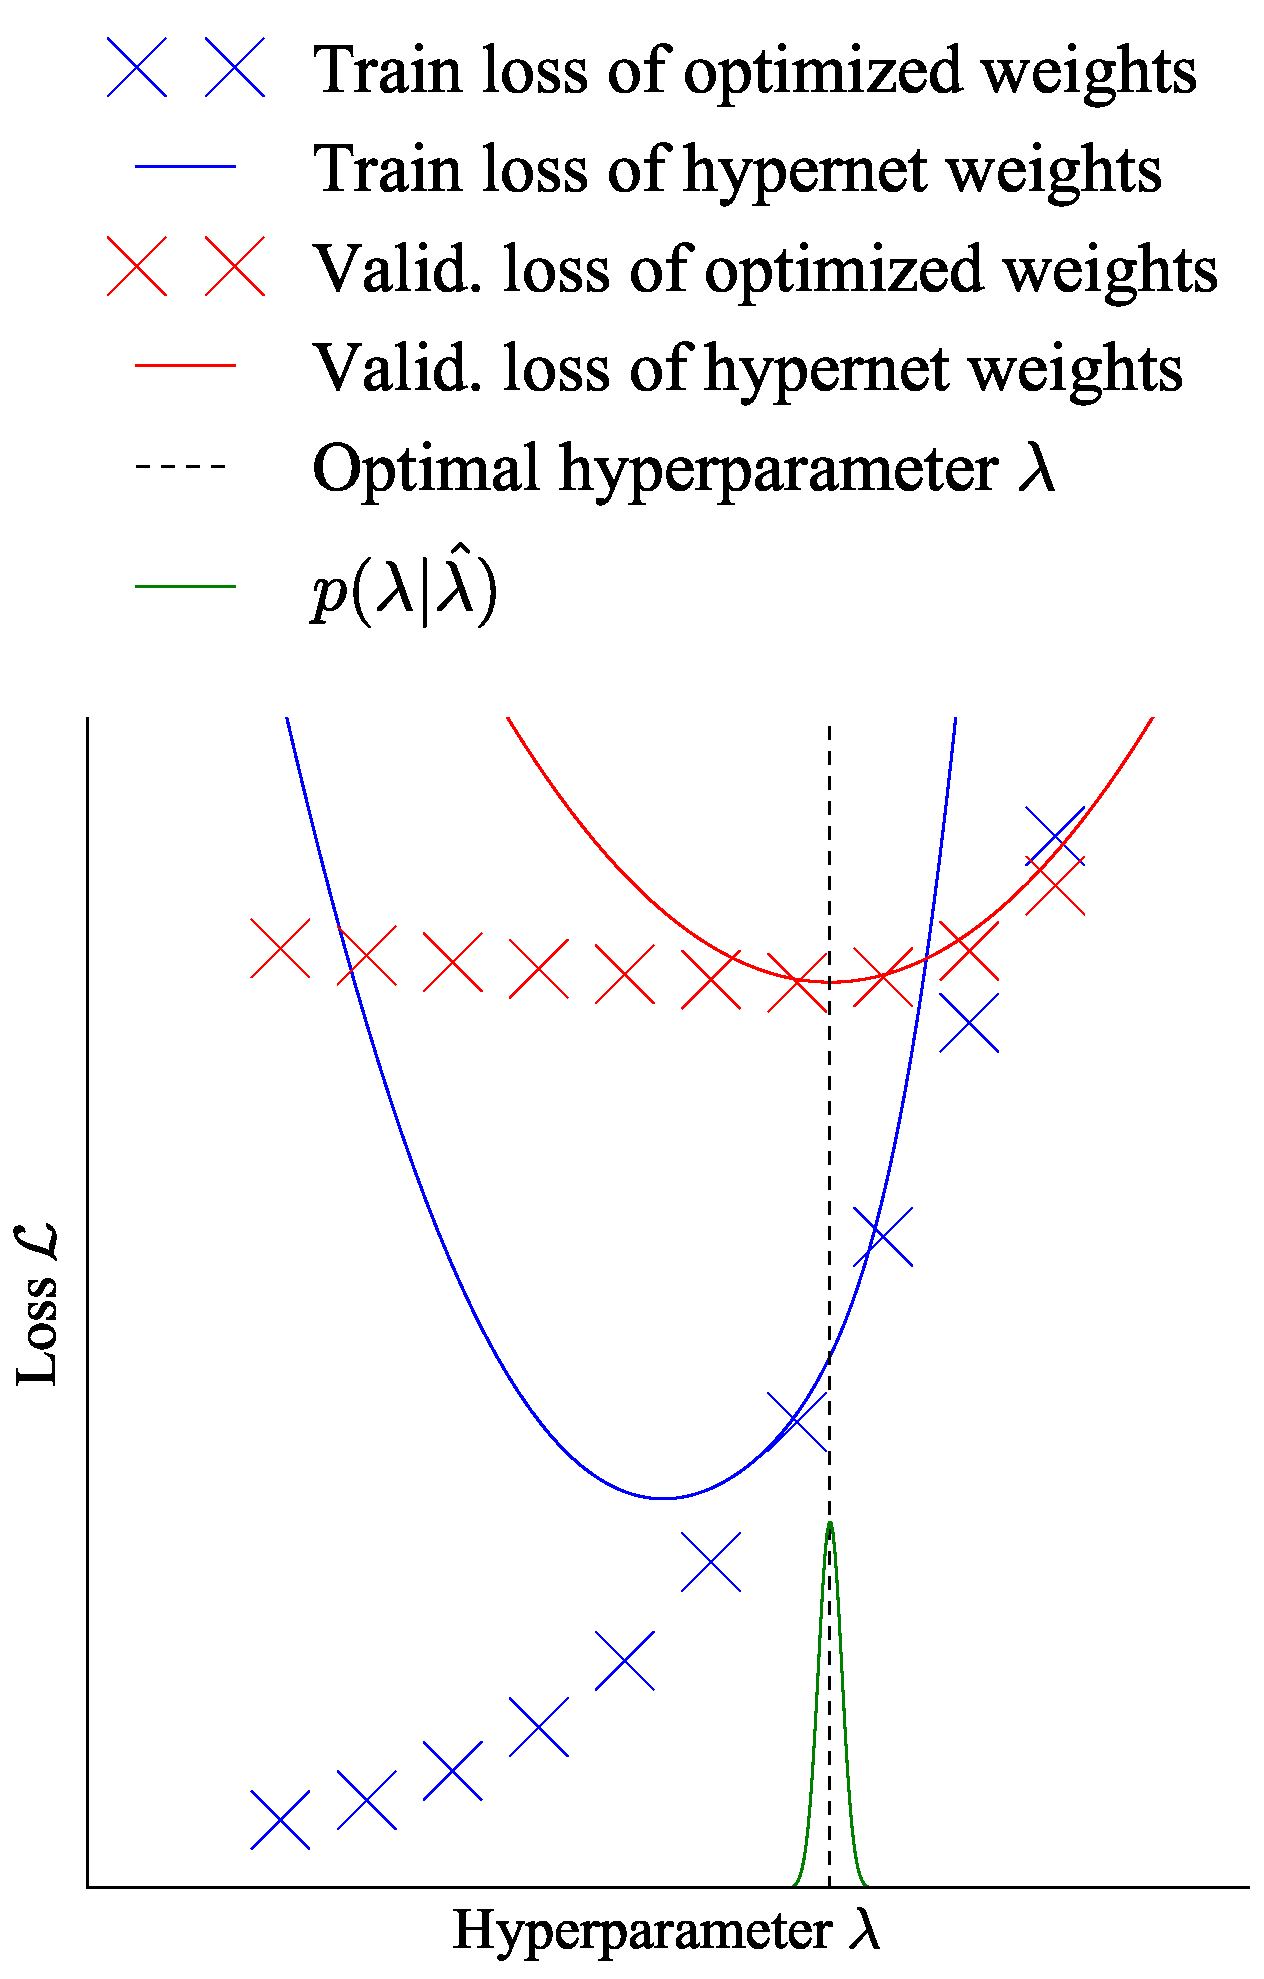
\includegraphics[trim={0 22cm 0 0},clip,height=7cm]{figures/hypernets_local_small.pdf}
	%\vspace{-0.33cm}
	\caption{
	Training and validation loss of a neural net for linear regression on MNIST, estimated by cross-validation (crosses) or by a hypernet (lines), which outputs $7,850$-dimensional network weights. 
	The training and validation loss can be cheaply evaluated at any hyperparameter value using a hypernet.
	Standard cross-validation requires training from scratch each time.
	\emph{Left:} A global approximation the best-response.
	\emph{Right:} A local approximation to the best-response.
	%\label{fig:exp1}
	}
\end{center}
\end{minipage}
\vphantom{A}


\mysection{Hyperparameter Tuning is Nested Optimization}
\newcommand{\hyper}{\lambda} %A variable hyper parameter.
\newcommand{\param}{\mathrm{w}} %The model parameters.
\newcommand{\innerLoss}[2]{\lossSymbolInner \! \left( #1, #2 \right)} %The loss function for the inner optimization. (1) The model parameters or the hypernets output. (2) A variable hyper parameter, or a fixed hyper parameter.
\newcommand{\innerOpt}{\argmin_{\param} \innerLoss{\param}{\hyper}} %The result of the inner optimization. 
\newcommand{\outerLoss}[1]{\lossSymbolOuter \! \left( #1 \right)}%, \hyperHyper \right)} %The loss function for the outer optimization. (1) The optimal model parameters, or the inner optimization.
\newcommand{\outerOpt}[1]{\argmin_{\hyper} \outerLoss{#1}} %The result of the inner optimization. (1) The optimal model parameters, or the inner optimization.
%
\newcommand{\lossSymbol}{\mathop{\mathcal{L}}} %The symbol to use for loss functions.
\newcommand{\lossSymbolInner}{\lossSymbol_{\mathrm{Train}}} %The symbol to use for the inner loss functions.
\newcommand{\lossSymbolOuter}{\lossSymbol_{\mathrm{Valid.}}} %The symbol to use for the outer loss functions.
\newcommand{\innerOptParam}[1]{\param^{*} \! \left( #1 \right)} %The optimal parameters of the model for the inner optimization. (1) Variable hyper parameters or fixed hyper parameters.

\begin{itemize}
	\item  Selecting a hyperparameter is finding a solution to the following bi-level optimization problem:
	\begin{align}
		\outerOpt{\innerOpt}
	\end{align}\\
	\item  The optimized model weights depend on the choice of hyperparameter.  This is a best-response function of the weights to the hyperparameters:
	\begin{align}
		\innerOptParam{\hyper} = \innerOpt
	\end{align}
\end{itemize}
\vphantom{A}


\mysection{Learning a Mapping from Hyperparameters to Optimal Weights}
\newcommand{\rename}[1]{#1'}
\newcommand{\EhyperFix}[1]{\mathop{\mathbb{E}}_{p \left( \rename{\hyper} \right)} \! \left[ #1 \right]}
\newcommand{\responseParam}{\phi} %The parameters of the response function. 
\newcommand{\argminTargetFix}{\responseParam}
\newcommand{\hyperSupport}{\mathrm{support} \! \left( \phyper \right)} %\phyper
\newcommand{\hyperDomain}{\textnormal{for all } \hyper \in \hyperSupport}
\newcommand{\phyper}{p \left( \hyper \right)}
\newcommand{\proofLossFix}{\innerLoss{\approxResponse{\rename{\hyper}}{\responseParam}}{\rename{\hyper}}}
\newcommand{\approxResponseSymbol}[1]{\param_{#1}} %The symbol for the approximate response function. (1) A variable hypernet, or a fixed hypernet.
\newcommand{\approxResponse}[2]{\approxResponseSymbol{#2} ( #1 )} %The approximate response function. (1) A variable hyperparameter or fixed hyperparameter. (2) A variable hypernet, or a fixed hypernet.

\begin{itemize}
	\item A hypernet is a neural network which outputs network weights.
	\item The best-response takes hyperparameters and outputs weights, so approximate it with a hypernet.
	\begin{theorem*}
		Sufficiently powerful hypernets can learn continuous best-response functions, which minimizes the expected loss for any hyperparameter distribution.
		\begin{align*}
			\textnormal{There exists } \responseParam^{*}, \textnormal{ such that }&\hyperDomain, \\
			\innerLoss{\param_{\responseParam^{*}} \left( \hyper \right)}{\hyper} &= \min_{\param} \innerLoss{\param}{\hyper} \\
			\textnormal{and }\responseParam^{*} = \argmin_{\argminTargetFix} &\EhyperFix{\proofLossFix}
		\end{align*}
	\end{theorem*}
\end{itemize}


\newpage 
\mysection{Globally Optimizing the Hypernet}
\newcommand{\curRename}[1]{\smash{\hat{#1}}} %Rename the current lambdas for algLocal
\newcommand{\variableData}{\bf{x}} % A variable data point
\newcommand{\prior}[1]{p \left( #1 \right)} % The prior belief distribution of a variable. (1) A parameter or hyper parameter.
%\newcommand{\x}{x} %A variable data point.
\newcommand{\hyperDist}{\prior{\hyper}} %The distribution of hyper parameters.
\newcommand{\lossTrainData}[2]{\lossSymbolInner ( \variableData, #1, #2 )} %The loss from predictions of the model. (1) Training or Testing or data point.
\newcommand{\lossValidData}[1]{\lossSymbolOuter ( \variableData, #1)} %The loss from predictions of the model. (1) Training or Testing or data point.

\begin{itemize}
	\item We can learn the best-response without viewing pairs of hyperparameters and optimized weights, by substituting the hypernet output into the training loss.  The algorithm is denoted Hyper Training.
	\\
	\begin{algorithmic}[1]
	\State $\textnormal{initialize } \responseParam$
	\State $\textrm{initialize } \curRename{\hyper}$
	\For{$T_{\mathrm{hypernet}}$ steps}
		\State $\variableData \sim \textnormal{Training data}$, $\hyper \sim \hyperDist$
		\State $\responseParam = \responseParam - \alpha \nabla_{\responseParam}\lossTrainData{ \approxResponseSymbol{\responseParam}( \hyper )}{\hyper}$
	\EndFor
	\For{$T_{\mathrm{hyperparameter}}$ steps}
		\State $\variableData \sim \textnormal{Validation data}$
		\State $\curRename{\hyper} = \curRename{\hyper} - \beta \nabla_{\curRename{\hyper}} \lossValidData{\approxResponse{\curRename{\hyper}}{\responseParam}}$
	\EndFor \\
	\Return{$\curRename{\hyper}, \approxResponseSymbol{\responseParam} ( \curRename{\hyper} )$}
	\end{algorithmic}
\end{itemize}
\vphantom{A}

\mysection{Locally Optimizing the Hypernet}
\begin{itemize}
	\item It is difficult to learn the best-response globally due to finite network size and training time.
	\item It is easier to learn the best-response locally, update the hyperparameters and repeat.
	\\
	\begin{algorithmic}[1]
	\State $\textrm{initialize } \responseParam, \curRename{\hyper}$
	\For{$T_{\mathrm{joint}}$ steps}
		\State $\variableData \sim \textnormal{Training data}$, $\hyper \sim p ( \hyper | \curRename{\hyper} )$
		\State $\responseParam = \responseParam - \alpha \nabla_{\responseParam} \lossTrainData{\approxResponse{\hyper}{\responseParam}}{\hyper}$ 
		\State $\variableData \sim \textnormal{Validation data}$
		\State $\curRename{\hyper} = \curRename{\hyper} - \beta \nabla_{\curRename{\hyper}} \lossValidData{\approxResponse{\curRename{\hyper}}{\responseParam}}$
	\EndFor \\
	\Return{$\curRename{\hyper}, \approxResponse{\curRename{\hyper}}{\responseParam}$}
	\end{algorithmic}
\end{itemize}
\vphantom{A}

\mysection{Optimizing 7,850 Hyperparameters}
\newcommand{\hyperDimMedium}{10} %The dimensionality of the hyperparameter space for the medium dimensionality hyperparameter experiment.

\newcommand{\hyperDimLarge}{7,850}
\begin{itemize}
	\item We investigate our methods performance on tuning hyperparameters of dimensionality $\hyperDimMedium$ and $\hyperDimLarge$.\\\\
	\begin{tabular}{cc}
	Optimizing $\hyperDimLarge$ hyperparameters & Optimizing $\hyperDimMedium$ hyperparameters\\
	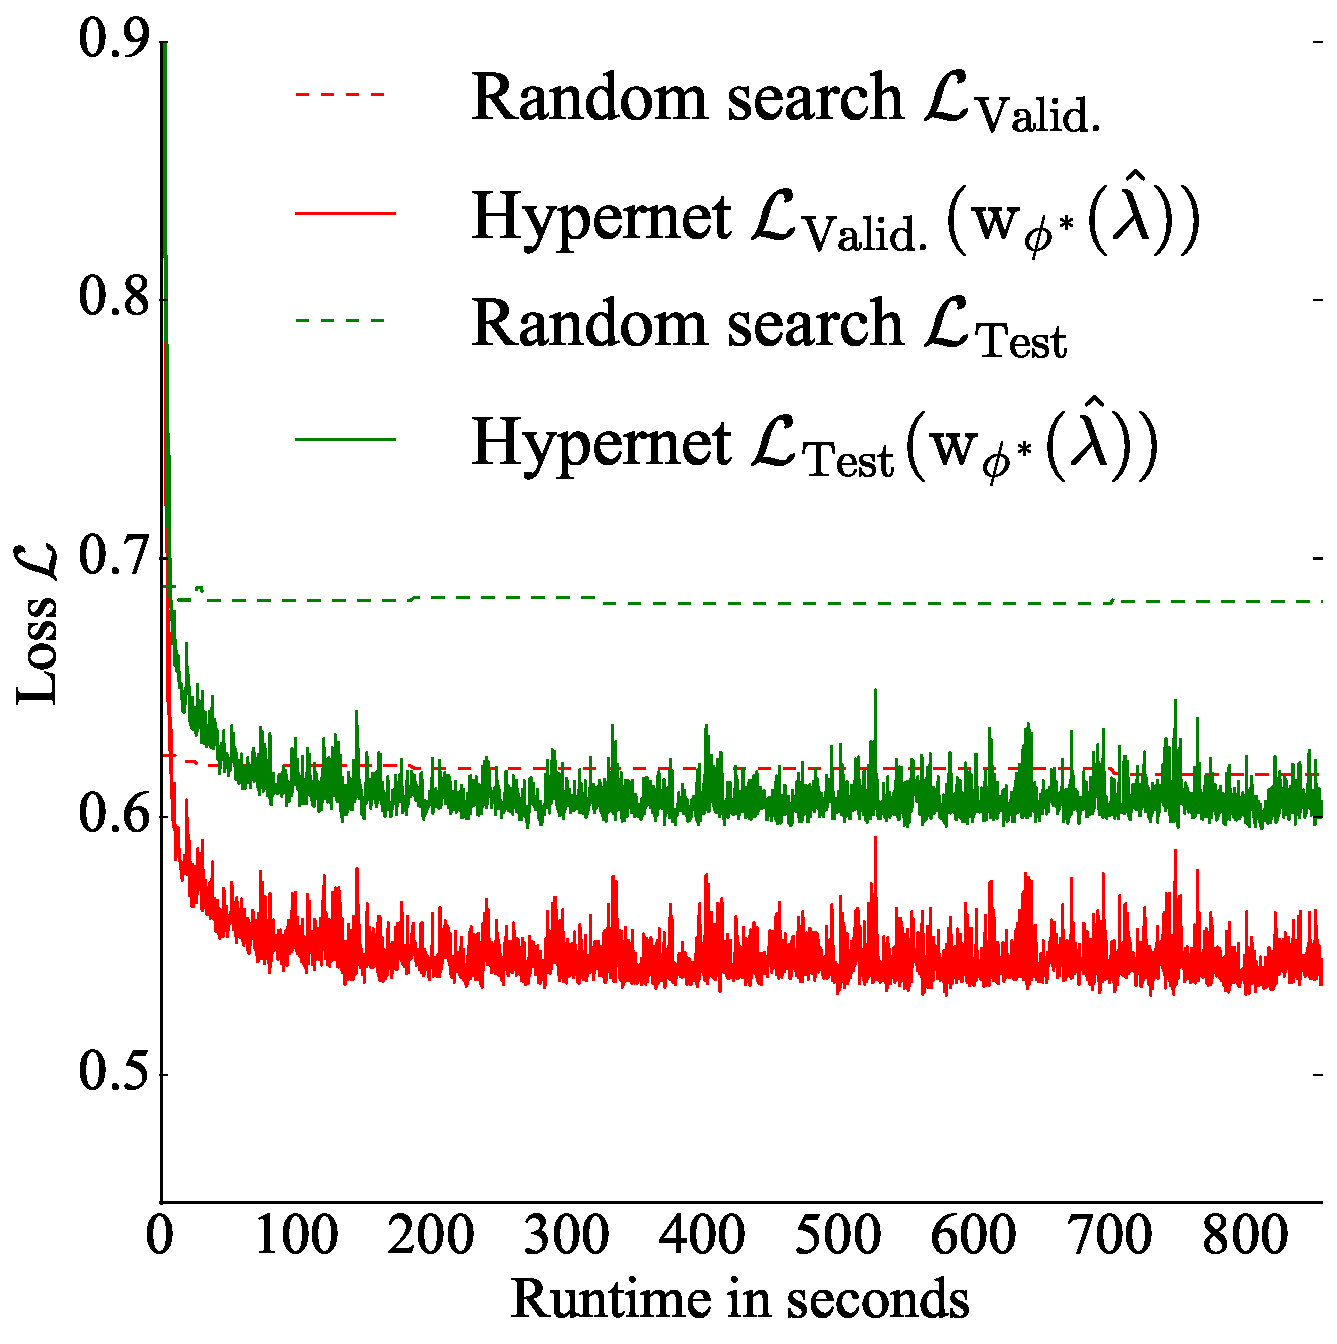
\includegraphics[width=17cm]{figures/hypernets_local_large.pdf} &
	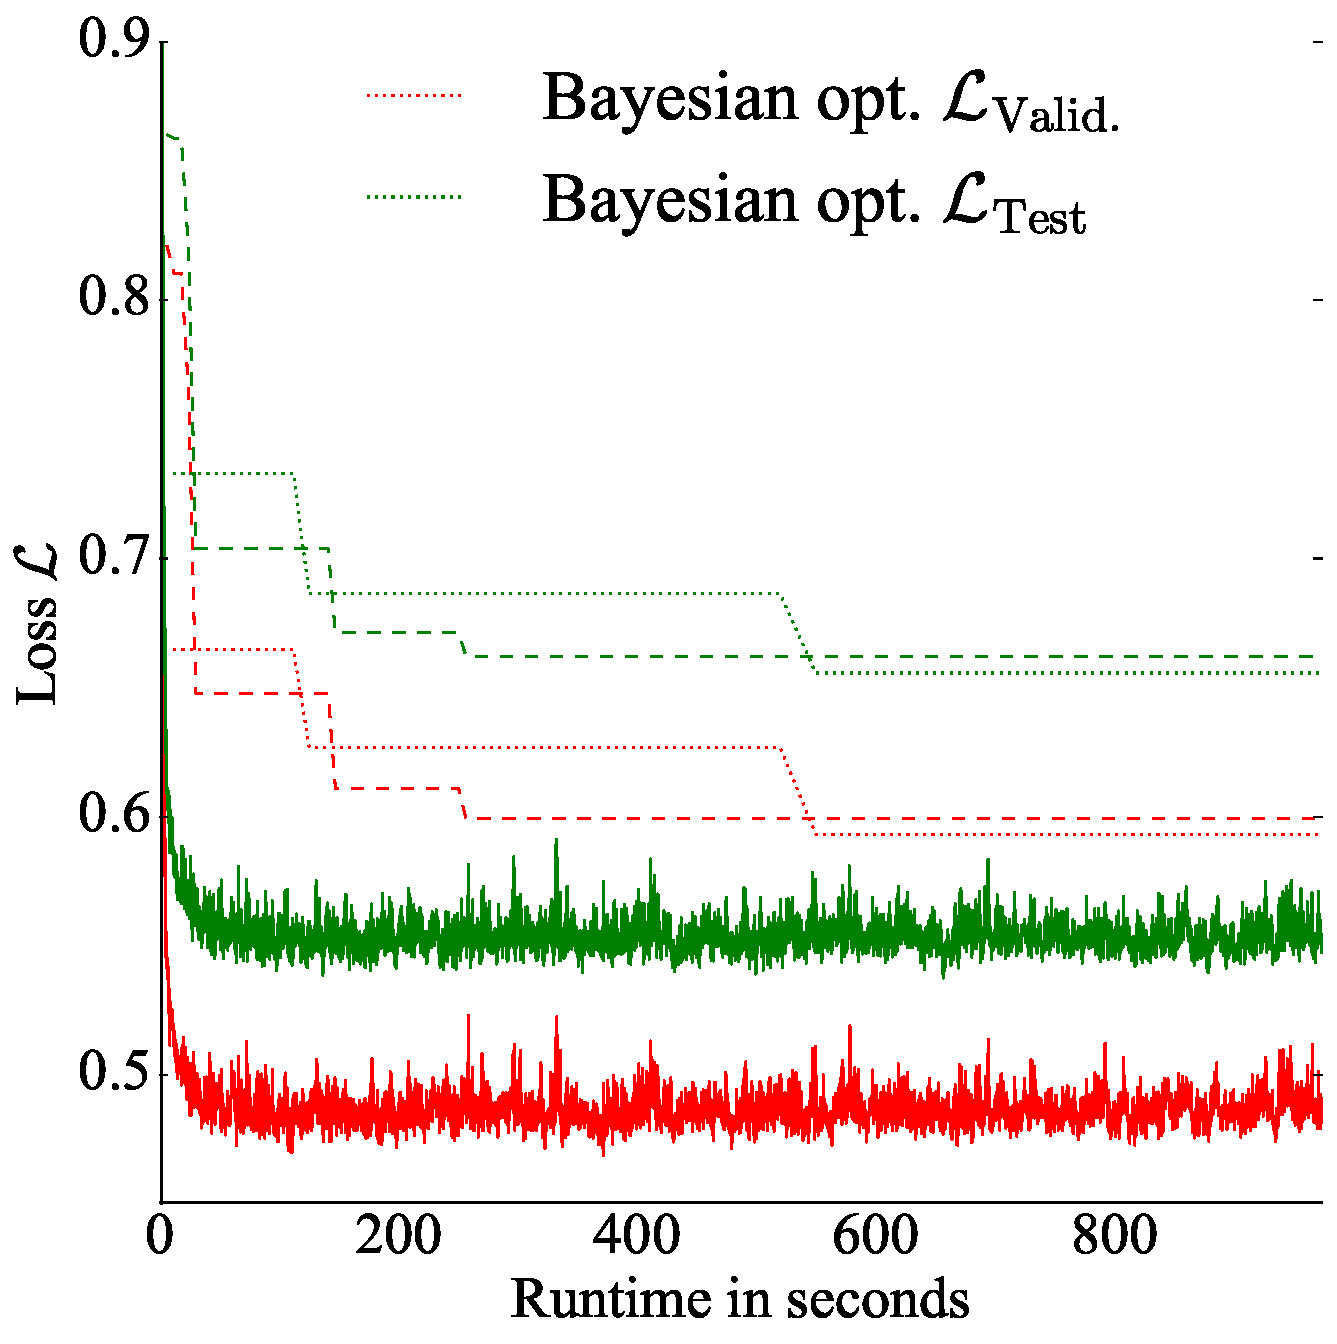
\includegraphics[width=17cm]{figures/hypernets_local_medium.pdf}
	\end{tabular}
\end{itemize}


\newpage
\mysection{Benefits of Hyper Training}
\begin{itemize}
	\item Our method provides two potential benefits.  These are a better inductive bias by learning the weights instead of loss, and viewing many hyperparameter settings during training.
	\item We analyze this by comparing our algorithm to Bayesian optimization with 25 samples and a hypernet trained on the same 25 samples.
\end{itemize}
\vphantom{A}
\begin{minipage}[c]{36cm}
\begin{center}
  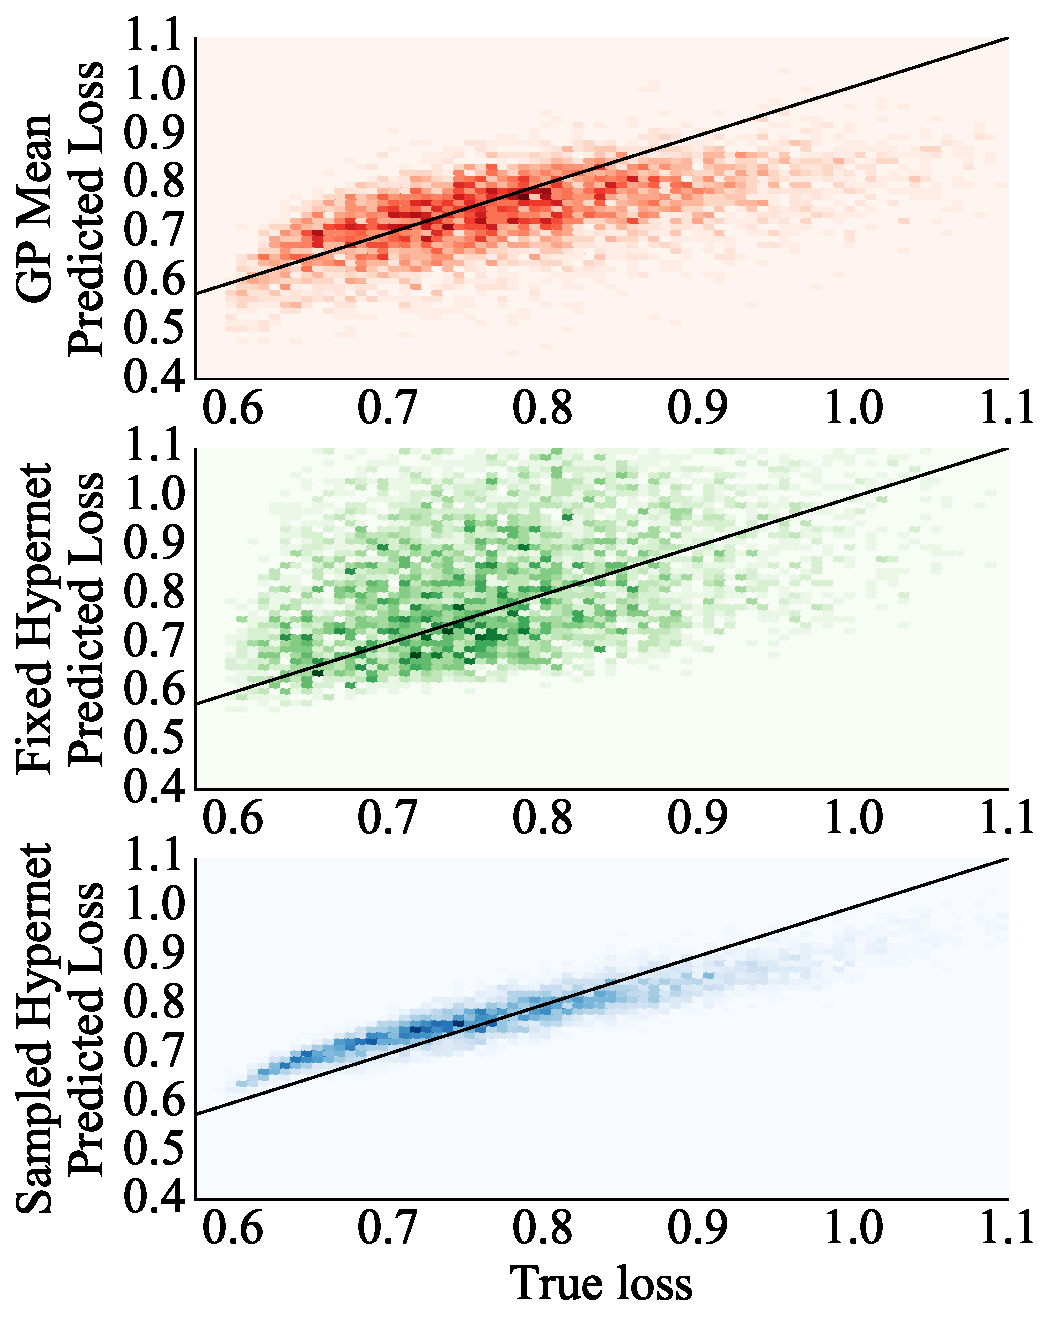
\includegraphics[height=21cm]{figures/learn_vs_true_loss_scatter.pdf}
  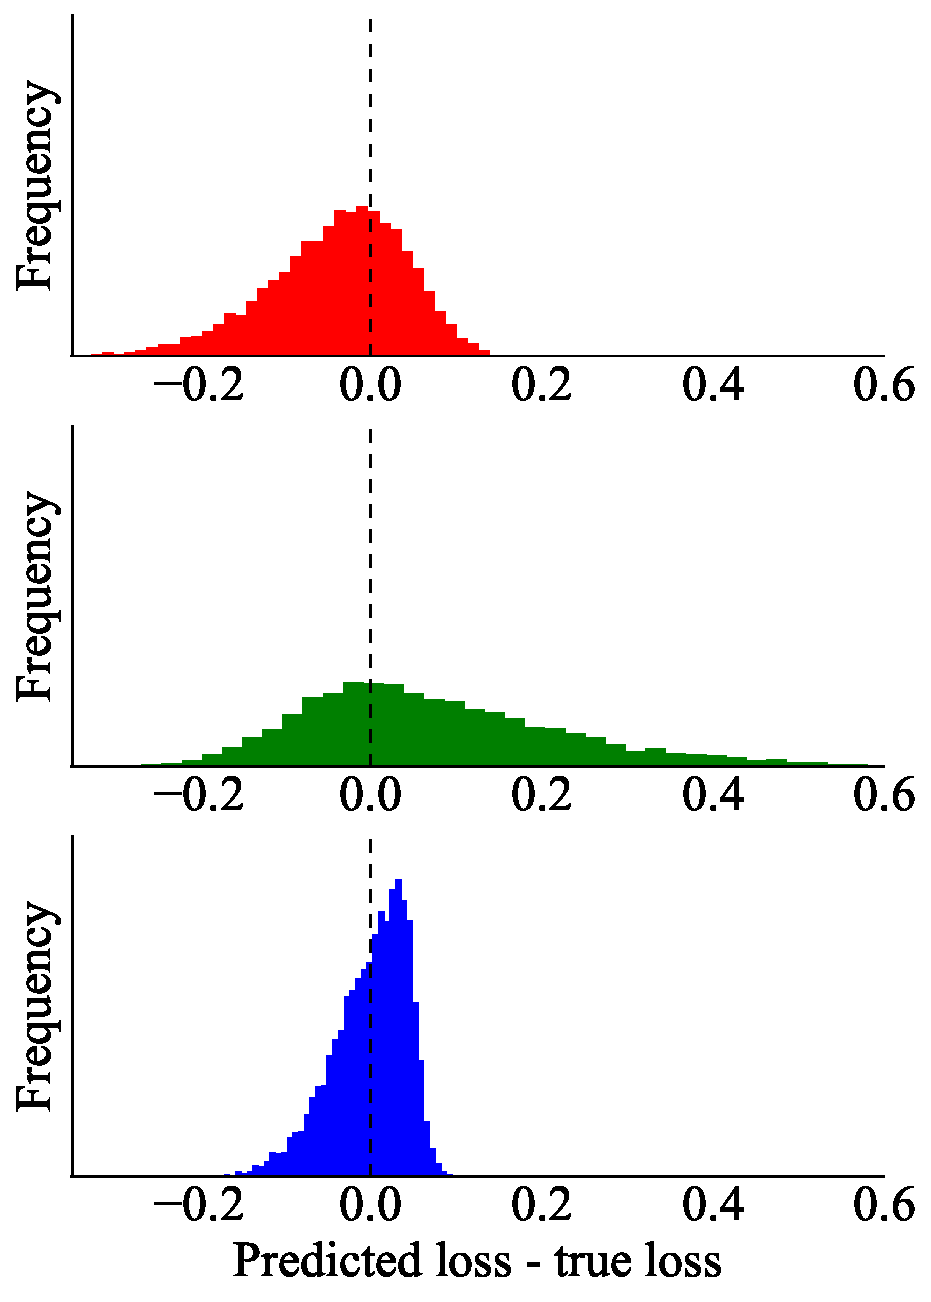
\includegraphics[height=21cm]{figures/learn_vs_true_loss_hist.pdf}
	%\vspace{-0.73cm}
	\caption{
	Comparing three approaches to predicting validation loss.
	\emph{First row:} {\color{red}A Gaussian process}, fit on a small set of hyperparameters and the corresponding validation losses.
	\emph{Second row:} {\color{green}A hypernet, fit on the same small set of hyperparameters} and the corresponding optimized weights.
	\emph{Third row:} Our proposed method, {\color{blue}a hypernet trained with stochastically sampled hyperparameters}.
	\emph{Left:}
	The distribution of predicted and true losses. 
	The diagonal black line is where predicted loss equals true loss. 
	\emph{Right:}
	The distribution of differences between predicted and true losses. 
	The Gaussian process often under-predicts the true loss, while the hypernet trained on the same data tends to over-predict the true loss.
	% while Algorithm~\ref{algLocal} is more sharply centered on 0.
	\label{fig:exp5}
	}
\end{center}
\end{minipage}
\vphantom{A}

\mysection{Conclusions}
\begin{itemize}
	\item We presented an algorithm that efficiently learns a differentiable approximation to a best-response for hyperparameter optimization.
	\item Hypernets can provide a better inductive bias for hyperparameter optimization than Bayesian optimization.
\end{itemize}

\begin{minipage}[c]{36cm}
\begin{center}
  	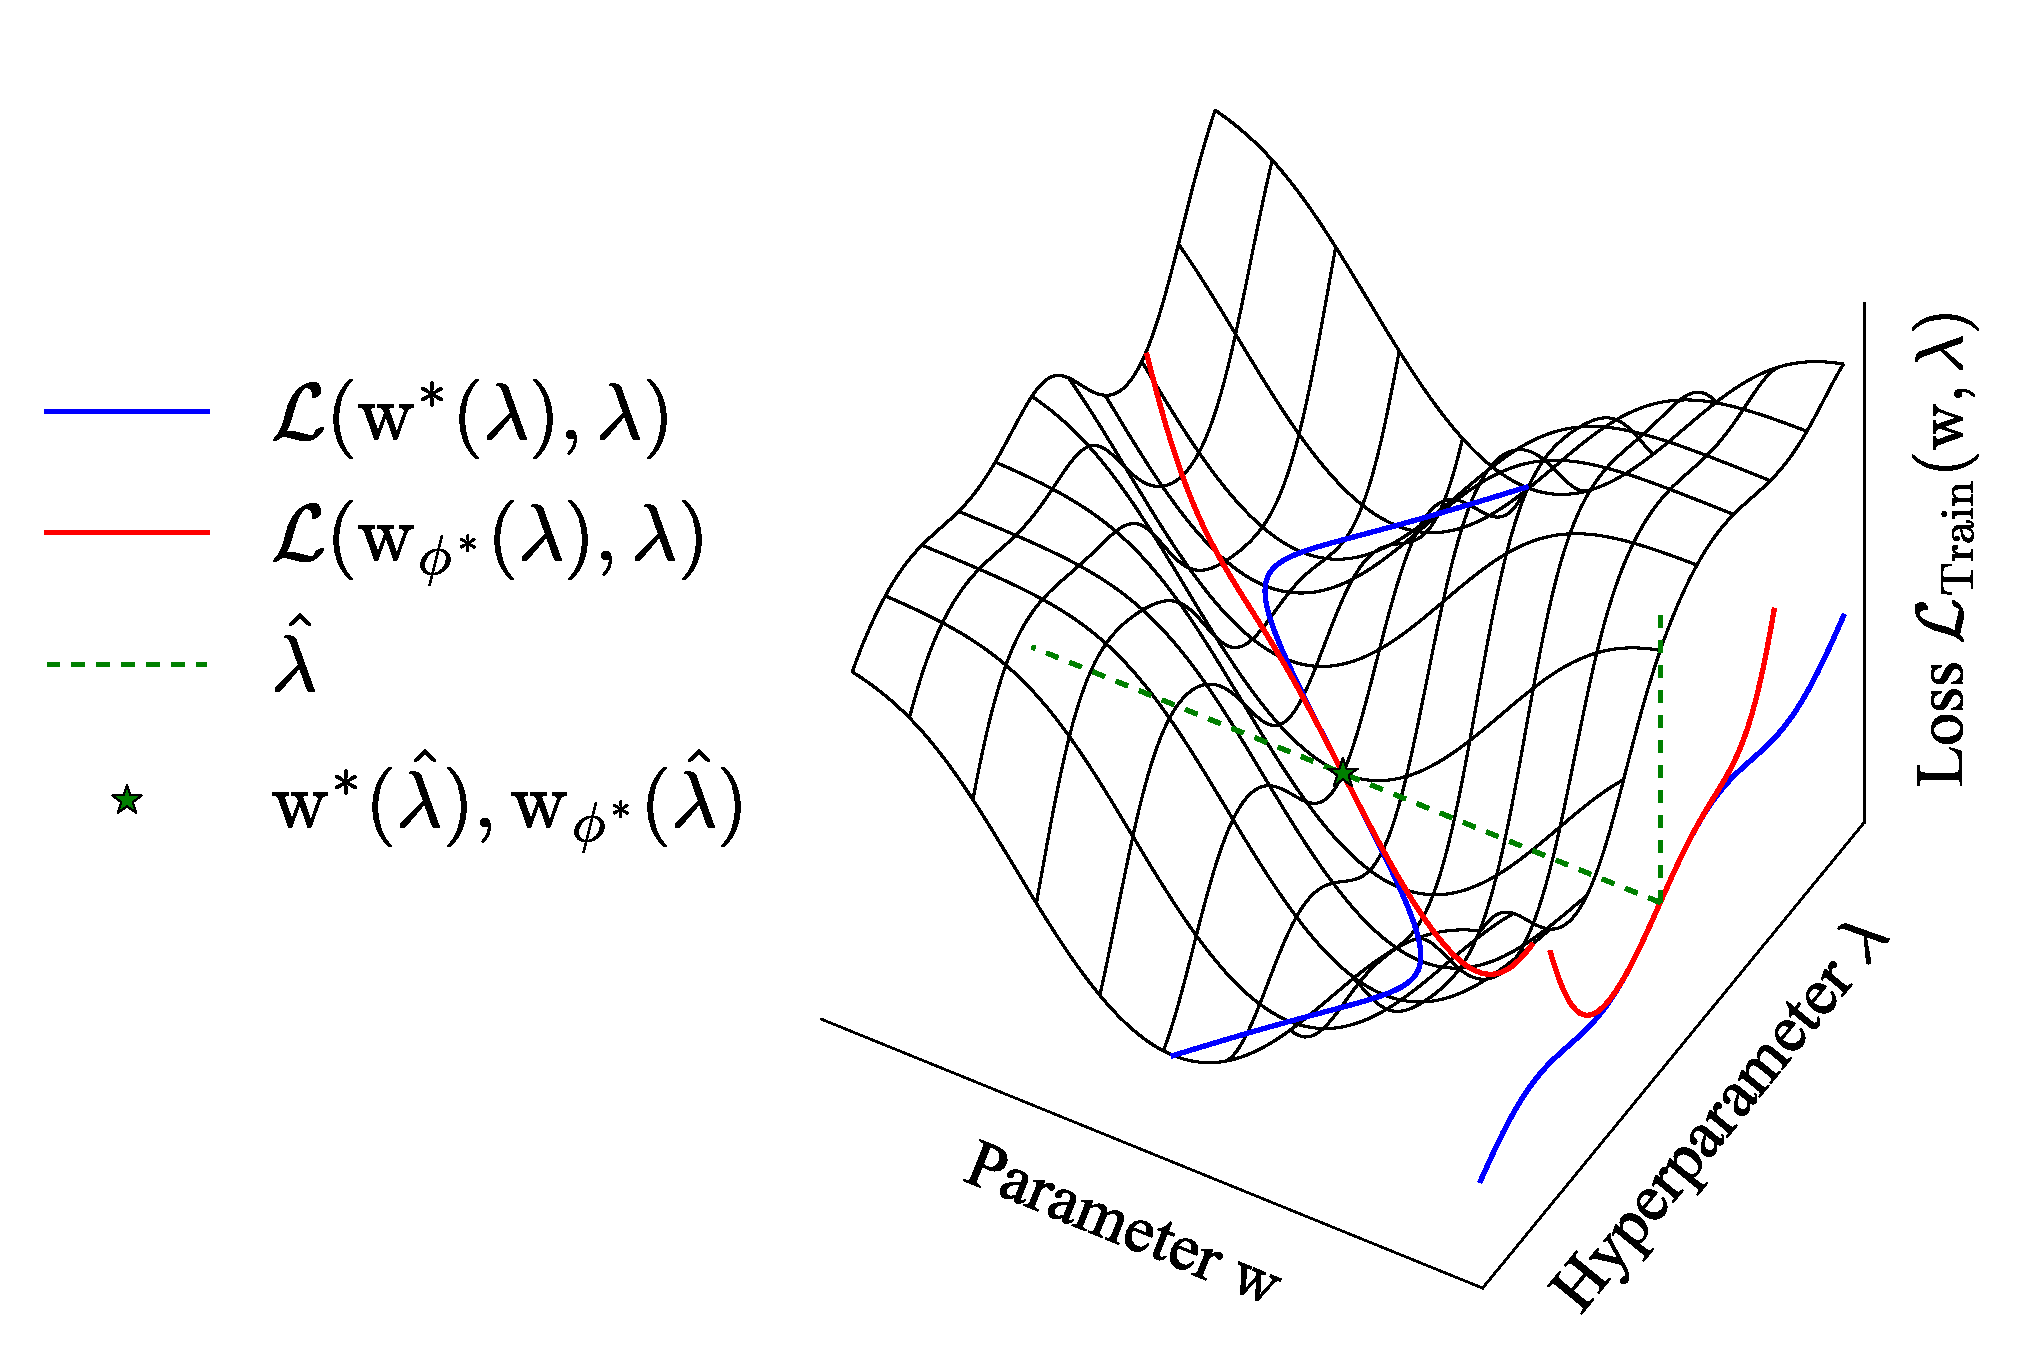
\includegraphics[width=17.5cm]{figures/train_loss_manifold.pdf}
	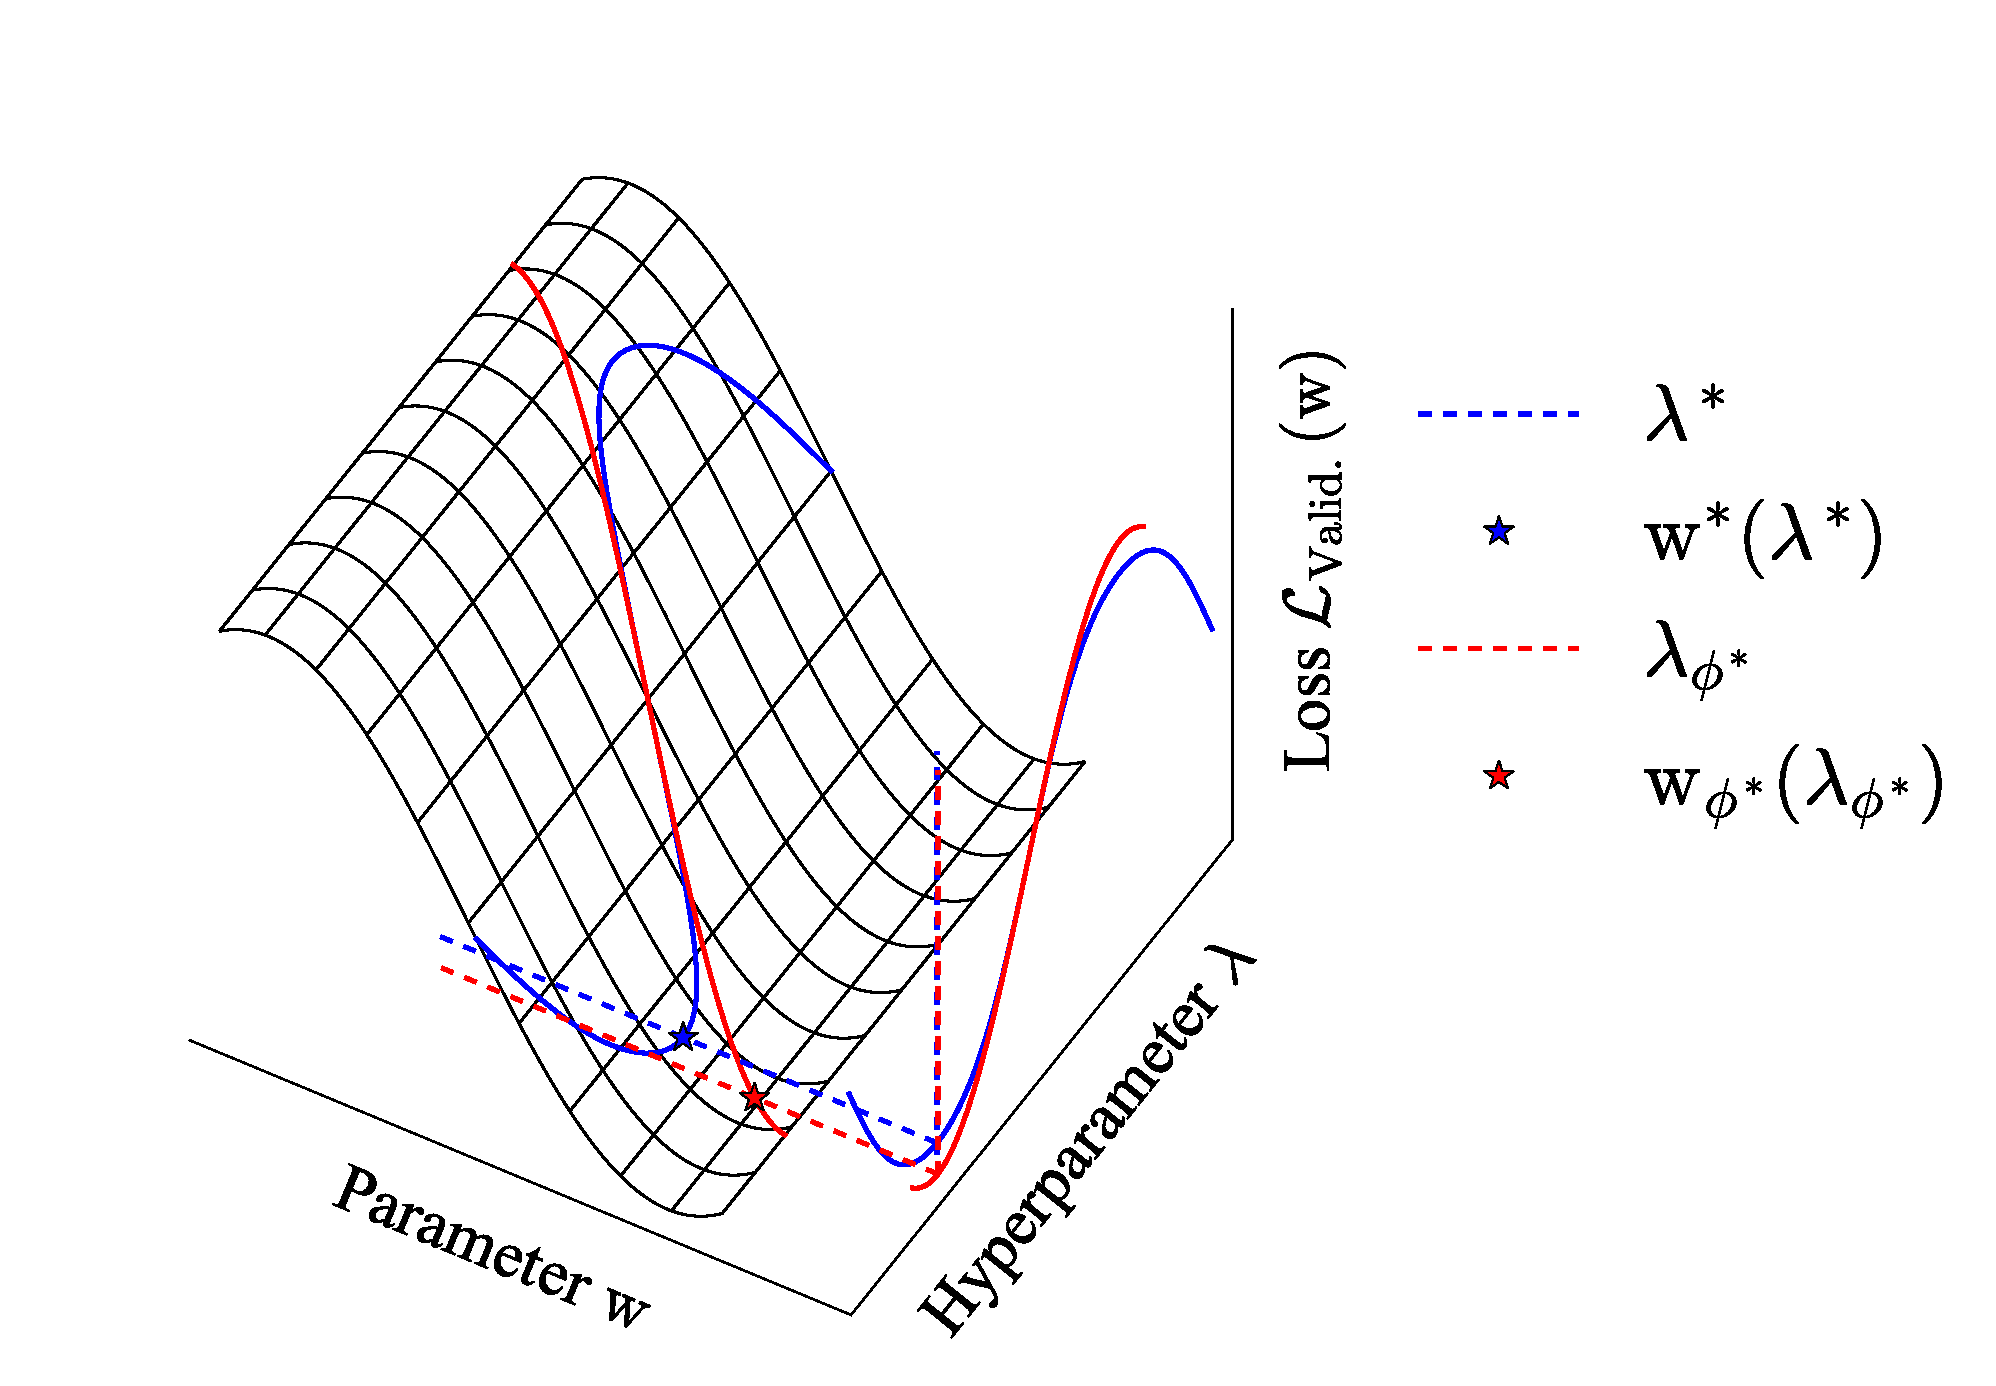
\includegraphics[width=17.5cm]{figures/valid_loss_manifold.pdf}
	\caption{
	A visualization of exact ({\color{blue} blue}) and approximate ({\color{red}red}) optimal weights as a function of given hyperparameters.
	\emph{Left:} The training loss surface. %, the best-response , and an approximate best-response . 
	\emph{Right:} The validation loss surface. %of the hyperparameter given the responses. 
	The approximately optimal weights $\param_{\phi^{*}}$ are output by a linear model fit at $\curRename{\lambda}$. %, while $\param^{*}$ is a best-response. 
	The true optimal hyperparameter is $\lambda^{*}$, while the hyperparameter estimated using approximately optimal weights is nearby at $\lambda_{\phi^{*}}$. %of the linearized best-response.
	\label{fig:theory1}
	}
\end{center}
\end{minipage}


\raggedright

\begin{tabular}{cc}
\begin{minipage}[c]{0.8\columnwidth}

%Code and paper at \texttt{https://github.com/lorraine2/hyperOpt2017}

\end{minipage}
\end{tabular}
%
%
%
\end{multicols}
\end{poster}

\end{document}

